\documentclass[../../FisicaTeorica.tex]{subfiles}

\begin{document}

\subsection{Gli autostati del momento angolare}
Concentriamoci sul caso particolare del momento angolare \q{analogo al caso classico} $\vec{J}=\vec{L} = \vec{X}\land \vec{P}$, che chiamiamo \textit{momento angolare orbitale}.\\

Vogliamo trovare la forma esplicita degli autoket $\ket{l,m}$ comuni a $\vec{L}^2$ e $L_3$, con $L\in \bb{N}$ (e non $\bb{N}/2$, dato che per $\vec{L}$ \q{classico} una rotazione di $2\pi$ è \textit{equivalente} a una rotazione nulla), e $|m| \leq l$. In effetti, se riusciamo a dimostrare l'esistenza di $\ket{l,l}$ (trovandolo esplicitamente) abbiamo automaticamente l'esistenza di tutti i altri autovettori, data la possibilità di \textit{costruirli} tramite $L_\pm$, e se l'insieme di tutti i tali autovettori è una base di $L^2$ abbiamo mostrato anche che lo spettro $\sigma(\vec{L}^2, L_z)$ è puramente \textit{discreto}.\\

Conviene allora partire esprimendo gli operatori che ci servono, ossia $L_3$ e $L_\pm$ (da cui si ricava anche $\vec{L}^2$), in coordinate \q{compatibili} con la simmetria rotazionale che stiamo studiando, ossia le \textbf{coordinate polari} $\{r,\theta,\varphi\}$.\\
 
Ricordiamo il passaggio da coordinate sferiche a cartesiane e viceversa:\marginpar{1. $L_3, L_\pm, L^2$ in coordinate polari}
\begin{align*}
\begin{cases}
x = r\sin\theta \cos \varphi\\
y = r\sin\theta \sin\varphi\\
z = r\cos\theta
\end{cases} \Leftrightarrow 
\begin{cases}
r = \sqrt{x^2 + y^2 +z^2}\\
\cos\theta = \displaystyle\frac{z}{\sqrt{x^2 + y^2 + z^2}}\\
\tan\varphi = \displaystyle \frac{y}{x}
\end{cases}
\end{align*}
Dato che $L_3$ e $L_\pm$ in rappresentazione $\{\vec{x}\}$ contengono le derivate $\partial_x$, $\partial_y$, $\partial_z$, conviene ricavarsi anche la trasformazione delle basi degli spazi \textit{tangenti} dalle coordinate cartesiane a quelle polari e viceversa\footnote{L'idea è che il cambio di coordinate oltre a trasformare anche i \textit{punti} di $\bb{R}^3$, trasforma anche i \textit{vettori}, che precisamente vanno intesi come appartenenti allo \textit{spazio tangente} a $\bb{R}^3$ in un dato punto (che nel caso di $\bb{R}^n$, agli effetti, coincide - cioè è \textit{canonicamente isomorfo} - con $\bb{R}^n$ stesso). Tali vettori sono \textit{combinazioni lineari} degli elementi della base dello spazio tangente, che è data (nel caso canonico in coordinate locali) proprio dalle \textit{derivazioni} $\partial/\partial_x$, $\partial/\partial_y$, $\partial/\partial_z$}. Procedendo direttamente dalla \textit{chain-rule}:
\begin{align}
\label{eqn:partial-phi}
\frac{\partial}{\partial \varphi} &=\frac{\partial x}{\partial \varphi}\frac{\partial}{\partial x} + \frac{\partial y}{\partial \varphi}\frac{\partial}{\partial y} + \frac{\partial z}{\partial \varphi}\frac{\partial}{\partial z} =\\ \nonumber
&= -r\sin\theta\sin\varphi\frac{\partial}{\partial x} + r\sin\theta \cos\varphi \frac{\partial}{\partial y} =\\ \nonumber
&= -y\frac{\partial}{\partial x} + x\frac{\partial}{\partial y}
\end{align}
E tale derivazione ci basta per esprimere $L_3$ in coordinate polari:
\begin{align*}
L_3 = -i\hbar x \frac{\partial}{\partial y}+ i\hbar y \frac{\partial}{\partial x} = -i\hbar \left(
x\frac{\partial}{\partial y} -y\frac{\partial}{\partial x}
\right) = \frac{\hbar}{i}\frac{\partial}{\partial \varphi}
\end{align*}

Per $L_{\pm}$ è invece necessario un po' più di lavoro\footnote{Si tratta di quel genere di conti che è bene fare almeno una volta nella vita!}. Partendo alla \textit{chain-rule} vista in (\ref{eqn:partial-phi}), notiamo che possiamo scrivere la $i$-esima derivata rispetto alle coordinate sferiche come prodotto scalare tra il vettore delle derivazioni rispetto alle coordinate cartesiane e la $i$-esima riga della \textit{trasposta} della matrice jacobiana del cambiamento di coordinate. Esplicitamente:
\begin{align*}
\begin{pmatrix}
\frac{\partial}{\partial r}\\
\frac{\partial}{\partial \theta}\\
\frac{\partial}{\partial \varphi}
\end{pmatrix} = \left(\frac{\partial (x,y,z)}{\partial (r,\theta,\varphi)}\right)^T\begin{pmatrix}
\frac{\partial}{\partial x}\\
\frac{\partial}{\partial y}\\
\frac{\partial}{\partial z}
\end{pmatrix}= 
\begin{pmatrix}
\sin\theta \cos\varphi & \sin\theta\sin\varphi & \cos\theta\\
r\cos\theta \cos\varphi & r\cos\theta \sin\varphi & - r\sin\theta\\
-r\sin\theta \sin\varphi & r\sin\theta\cos\varphi & 0
\end{pmatrix}
\begin{pmatrix}
\frac{\partial}{\partial x}\\
\frac{\partial}{\partial y}\\
\frac{\partial}{\partial z}
\end{pmatrix}
\end{align*}
E per la relazione inversa è necessario invertire la matrice:
\begin{align}
\begin{pmatrix}
\frac{\partial}{\partial x}\\
\frac{\partial}{\partial y}\\
\frac{\partial}{\partial z}
\end{pmatrix} = \left[\left(\frac{\partial (x,y,z)}{\partial (r,\theta,\varphi)}\right)^T\right]^{-1} \begin{pmatrix}
\frac{\partial}{\partial r}\\
\frac{\partial}{\partial \theta}\\
\frac{\partial}{\partial \varphi}
\end{pmatrix}= 
\begin{pmatrix}
\sin\theta \cos\varphi & \frac{1}{r}\cos\theta\cos\varphi &- \frac{\sin\varphi}{r\sin\theta}\\
\sin\theta\sin\varphi & \frac{1}{r}\cos\theta\sin\varphi & \frac{\cos\varphi}{r\sin\theta}\\
\cos\theta & -\frac{\sin\theta}{r} & 0
\end{pmatrix}
\begin{pmatrix}
\frac{\partial}{\partial r}\\
\frac{\partial}{\partial \theta}\\
\frac{\partial}{\partial \varphi}
\end{pmatrix}
\label{eqn:relazione_inversa}
\end{align}



Ricaviamo allora:
\begin{align*}
L_\pm \equiv L_1 \pm iL_2 &= (X_2 P_3-X_3P_2)\pm i(X_3P_1 -X_1P_3)=\\
&=\left(-i\hbar y\frac{\partial}{\partial z}+i\hbar z \frac{\partial}{\partial y} \right) \pm i \left(-i\hbar z \frac{\partial}{\partial x} + i\hbar x \frac{\partial}{\partial x}\right)=\\
&=\hbar \left[-iy \hlc{Yellow}{\frac{\partial}{\partial z}} + i\hlc{SkyBlue}{z} \frac{\partial}{\partial y} \pm \hlc{SkyBlue}{z} \frac{\partial}{\partial x} \mp x\hlc{Yellow}{\frac{\partial}{\partial z}}\right]=\\
&=\hbar\left[\left(\mp x -iy\right)\frac{\partial}{\partial z} +z\left(\pm \frac{\partial}{\partial x}+i\frac{\partial}{\partial y}\right)\right]=\\
&=\hbar\left[\mp(x\pm iy)\frac{\partial}{\partial z} \pm z\left(\frac{\partial}{\partial x}\pm i \frac{\partial}{\partial y}\right)\right]
\end{align*}
Dalle equazioni del cambiamento di coordinate abbiamo le sostituzioni:
\begin{align*}
x \pm i y&= r(\sin\theta\cos\varphi \pm i \sin\theta\sin\varphi)=\\ &= r\sin\theta\hlc{ForestGreen}{(\cos\varphi \pm i\sin\varphi)}=r\sin\theta \hlc{ForestGreen}{e^{\pm i\varphi}}\\
z &= r\cos\theta
\end{align*}
Dopo le quali giungiamo a:
\begin{align*}
L_\pm &= \hbar \left[\mp r \sin\theta e^{\pm i\varphi}\frac{\partial}{\partial z} \pm r\cos \theta \left(\frac{\partial}{\partial x} \pm i \frac{\partial}{\partial y}\right) \right]
\end{align*}
Otteniamo le ultime sostituzioni da (\ref{eqn:relazione_inversa}):
\begin{align*}
\frac{\partial}{\partial z} &= \frac{1}{r}\left( r\cos\theta \frac{\partial}{\partial r} - \sin\theta\frac{\partial}{\partial \theta}\right)\\
\frac{\partial}{\partial x} \pm i\frac{\partial}{\partial y} &= \frac{1}{r}\Big [ r\sin\theta\left(\cos\varphi \pm i\sin\varphi\right) \frac{\partial}{\partial r} +\\
&\qquad +\cos\theta(\cos\varphi \pm i\sin\varphi)\frac{\partial}{\partial \theta} +\\
&\qquad +\frac{1}{\sin\theta}(-\sin\varphi \pm i\cos\varphi)\frac{\partial}{\partial \varphi}\Big] =\\
&=\frac{1}{r}e^{\pm i\varphi}\left(r\sin\theta \frac{\partial}{\partial r} + \cos\theta \frac{\partial}{\partial\theta}\pm \frac{i}{\sin\theta}\frac{\partial}{\partial \varphi}\right)
\end{align*}
Da cui, infine, giungiamo a:
\begin{align*}
L_\pm &= \hbar e^{\pm i\varphi} \left[
\mp \frac{\cancel{r}\sin\theta}{\cancel{r}}\left(\bcancel{r\cos\theta\frac{\partial}{\partial r}} -\sin\theta\frac{\partial}{\partial \theta}\right)
\pm \frac{\cancel{r}\cos\theta}{\cancel{r}} \left(\bcancel{r\sin\theta\frac{\partial}{\partial r}} +\cos\theta\frac{\partial}{\partial \theta}\pm\frac{i}{\sin\theta}\frac{\partial}{\partial \varphi} \right)
 \right] =\\
 &= \hbar e^{\pm i\varphi} \left[\pm \sin^2\theta\frac{\partial}{\partial \theta}
\pm \cos^2 \theta\frac{\partial}{\partial \theta} + i\cot\theta\frac{\partial}{\partial \varphi}
 \right ] =\\
 &= \hbar e^{\pm i\varphi} \left(i\cot\theta\frac{\partial}{\partial \varphi} \pm \frac{\partial}{\partial \theta}\right)
\end{align*}

Poiché anche $\vec{L}^{\,2}$ soddisfa la relazione vista per $\vec{J}^{\,2}$, possiamo scrivere:
\begin{align*}
\vec{L}^{\,2}&=L_+ L_- + L_3^2 -\hbar L_3 =\\
&=\hbar^2\left ( e^{i\varphi} \left(i \cot \theta \hlc{Yellow}{\frac{\partial}{\partial \varphi}}+\hlc{Yellow}{\frac{\partial }{\partial \theta}}\right)\left[e^{-i\varphi}\left(i \cot\theta \frac{\partial}{\partial \varphi}-\frac{\partial}{\partial \theta}\right)\right] -\frac{\partial^2}{\partial \varphi^2}+i\frac{\partial}{\partial \varphi}\right)
\end{align*}
\textbf{Attenzione!} Le derivate evidenziate si applicano a tutto ciò che è alla loro destra, e perciò purtroppo non vale usare il prodotto notevole:
\[
e^{i\varphi} \left(i \cot \theta \frac{\partial}{\partial \varphi}+{\frac{\partial }{\partial \theta}}\right)\left[e^{-i\varphi}\left(i \cot\theta \frac{\partial}{\partial \varphi}-\frac{\partial}{\partial \theta}\right)\right] 
\neq \left(i\cot \theta \frac{\partial}{\partial \varphi}\right)^2 - \frac{\partial^2}{\partial \theta^2}
\]
Per tale prodotto otteniamo invece:
\begin{align*}
&= ie^{i\varphi} \cot\theta \frac{\partial}{\partial \varphi} \left (e^{-i\varphi} \left( i\cot\theta \frac{\partial}{\partial \varphi}-\frac{\partial}{\partial \theta}\right)\right)
+ e^{i\varphi} \frac{\partial}{\partial \theta}\left(e^{-i\varphi} \left(i\cot\theta\frac{\partial}{\partial \varphi}-\frac{\partial}{\partial \theta}\right)\right)=\\
&=i\cancel{e^{i\varphi}}\cot\theta\left(-i\cancel{e^{-i\varphi}}\left(i\cot\theta \frac{\partial}{\partial\varphi}-\frac{\partial}{\partial \theta}\right) + \cancel{e^{-i\varphi}}\left(i\cot\theta \frac{\partial^2}{\partial \varphi^2}-\frac{\partial}{\partial \theta\partial \varphi}\right)\right)+\\
&+ \cancel{e^{i\varphi}}\cancel{e^{-i\varphi}}\left(-\frac{\partial^2}{\partial \theta^2} + i\cot\theta\frac{\partial}{\partial\varphi\partial \theta} -\frac{i}{\sin^2\theta}\frac{\partial}{\partial \varphi} \right) =\\
&= i\cot\theta \left( \cot\theta \frac{\partial}{\partial \varphi}+i\frac{\partial}{\partial \theta} + i\cot\theta \frac{\partial^2}{\partial \varphi^2} -\bcancel{\frac{\partial}{\partial \theta \partial \varphi}} \right) -\frac{\partial^2}{\partial \theta^2}+\bcancel{i\cot\theta \frac{\partial}{\partial \varphi\partial \theta}}-\frac{i}{\sin^2\theta}\frac{\partial}{\partial \varphi} =\\
&= i\cot^2\theta \frac{\partial}{\partial \varphi}-\cot\theta\frac{\partial}{\partial \theta}-\cot^2\theta\frac{\partial^2}{\partial \varphi^2} -\frac{\partial^2}{\partial \theta^2} -\frac{i}{\sin^2 \theta}\frac{\partial}{\partial \varphi}
\end{align*}
Sostituendo nell'espressione per $\vec{L}^2$ e raccogliendo i termini simili otteniamo:
\begin{align*}
\vec{L}^2 &= \hbar^2 \left [
-\frac{\partial^2}{\partial \theta^2} + i\left(\cot^2 \theta -\frac{1}{\sin^2 \theta}+1\right)\frac{\partial}{\partial \varphi} - (\cot^2 \theta +1) \frac{\partial^2}{\partial \varphi^2} -\cot\theta \frac{\partial}{\partial \theta}
\right]
\end{align*}
Ricordando la relazione goniometrica:
\begin{align*}
\cot^2 \theta =\frac{\cos^2 \theta}{\sin^2 \theta} =\frac{1-\sin^2\theta}{\sin^2\theta}=\frac{1}{\sin^2 \theta} -1
\end{align*}
possiamo semplificare le due parentesi tonde. Giungiamo infine a:
\begin{align*}
\vec{L}^2 = -\hbar^2 \left[\frac{1}{\sin^2\theta}\frac{\partial^2}{\partial \varphi^2} +\frac{\partial^2}{\partial \theta^2} + \cot\theta \frac{\partial}{\partial \theta} \right]
\end{align*}
Che possiamo \q{comprimere} ulteriormente applicando Leibniz \textit{al contrario}:
\begin{align*}
\frac{\partial^2}{\partial \theta^2} +\frac{\cos\theta}{\sin\theta}\frac{\partial}{\partial \theta} = \frac{1}{\sin\theta}\left(\cos\theta \frac{\partial}{\partial \theta} + \frac{\partial^2}{\partial \theta^2}\right)=\frac{1}{\sin\theta}\left(\frac{\partial}{\partial \theta} \sin\theta \frac{\partial}{\partial \theta}\right)
\end{align*}
E finalmente otteniamo:
\[
\vec{L}^{\,2}=-\hbar^2\left[ \frac{1}{\sin^2 \theta}\frac{\partial^2}{\partial \varphi^2}+\frac{1}{\sin\theta}\frac{\partial}{\partial \theta}\sin\theta \frac{\partial}{\partial \theta}\right]
\]

Vediamo che $L_3$, $L_\pm$ e $\vec{L}^2$ agiscono solo su $\theta$ e $\varphi$ e non su $r$. Possiamo allora usare l'isomorfismo \q{delle coordinate sferiche}:
\begin{align*}
L^2(\bb{R}^3, d^3x)\cong L^2(\bb{R}_+, r^2 dr)\otimes L^2(S^2, d\Omega = \sin\theta d\theta d\varphi)
\end{align*}
e cerchiamo le autofunzioni $f_{ln}(\theta,\varphi)$ di $\vec{L}^{\,2}$ e $L_3$ in $L^2(S^2, d\Omega)$ di autovalori rispettivamente $\hbar^2 l(l+1)$ e $\hbar m$, risolvendo le equazioni (differenziali) agli autovalori date da:
\begin{align}
L_3 f_{lm}(\theta,\varphi) &= \hbar m f_{lm}(\theta,\varphi)\label{eqn:autovalori-L_3}\\
\vec{L}^2 f_{lm}(\theta,\varphi) &= \hbar^2 l(l+1) f_{lm}(\theta,\varphi)\label{eqn:autoalori-Lquadro}
\end{align}
Utilizziamo una\marginpar{2. Autofunzioni fattorizzate} tecnica comune nella risoluzione di equazioni differenziali alle derivate parziali, che sta nel cercare soluzioni \textit{fattorizzabili} del tipo:
\begin{align*}
f_{lm}(\theta,\varphi) = \Theta_{lm}(\theta) \Phi_{lm}(\varphi)
\end{align*}
Sostituendo nella (\ref{eqn:autovalori-L_3}) otteniamo (sopprimendo temporaneamente gli indici $lm$ per alleggerire la notazione):
\begin{align*}
L_3 \Theta(\theta)\Phi(\varphi) = \frac{\bcancel{\hbar}}{i}\cancel{\Theta(\theta)}\frac{\partial}{\partial\varphi} \Phi(\varphi)=\bcancel{\hbar} m\cancel{ \Theta(\theta)}\Phi(\varphi)
\end{align*}
che è a variabili separabili, e conduce a:\marginpar{$\Phi(\varphi)$}
\begin{align*}
\frac{\Phi'(\varphi)}{\Phi(\varphi)} = im \Rightarrow \Phi(\varphi) \sim e^{im\varphi}
\end{align*}
Ricavare $\Theta_{lm}(\theta)$ richiede invece un po' più di conti. Partiamo notando che, poiché in $\vec{L}^2$ l'unica derivata rispetto a $\varphi$ è al quadrato, si ha che le $\Theta_{lm}(\theta)$ \textit{non} dipendono dal segno di $m$, ossia:
\begin{align*}
\Theta_{lm}(\theta)=\Theta_{l,-m}(\theta)=\Theta_{l,|m|}(\theta)
\end{align*}
Ciò si verifica applicando $\vec{L}^2$ ad un'autofunzione:
\begin{align*}
\vec{L}^2 \Theta(\theta)\Phi(\varphi) &= -\bcancel{\hbar^2}\left[\frac{1}{\sin^2 \theta}\frac{\partial^2}{\partial \varphi^2} + \frac{\partial^2}{\partial \theta^2} + \cot\theta\frac{\partial}{\partial \theta} \right] \Theta(\theta) e^{im\varphi} =\bcancel{ \hbar^2} l(l+1) \Theta(\theta)e^{im\varphi}=\\
&=-\cancel{e^{im\varphi}}\left(-\frac{m^2}{\sin^2 \theta} +\frac{\partial^2}{\partial \theta^2} + \cot\theta \frac{\partial}{\partial \theta} \right)\Theta(\theta)= l(l+1)\Theta(\theta) \cancel{e^{im\varphi}}
\end{align*}
E perciò $\Theta(\theta)$ dipende solo da $m^2$, e perciò non \q{avverte} cambiamenti di segno di $m$.\\
L'equazione differenziale appena ricavata è difficile da risolvere direttamente\footnote{Lo si può comunque fare, per esempio tramite metodi con \textit{serie di potenze}, come accennato qui: \url{http://www.eng.fsu.edu/~dommelen/quantum/style_a/nt_soll2.html}}, ma fortunatamente possiamo utilizzare i risultati ottenuti esaminando l'algebra di $\vec{L}$. Supponiamo infatti che esista un autoket $\ket{l,l}$ \q{massimo}, nel senso che $L_+$ non possa \q{alzarlo} ulteriormente, e tale che applicando ad esso $L_-$ iterativamente sia possibile ottenere \textit{tutti} gli altri autoket:\marginpar{$\Theta(\theta)$ tramite $L_+$}
\begin{align}
L_+ \ket{l,l}&=0 \label{eqn:autoket-max}\\
\ket{l,m} &\propto L_-^{l-m}\ket{l,l} \label{eqn:autoket-abbassato} \qquad (m>0)
\end{align}
 
Riscrivendo (\ref{eqn:autoket-max}) in rappresentazione in \textit{coordinate sferiche} $\{r,\theta,\varphi\}$ giungiamo a un'equazione differenziale a variabili separabili: 
\begin{align*}
&\cancel{\hbar e^{i\varphi}}\left(i\cot \theta \frac{\partial}{\partial \varphi}+\frac{\partial}{\partial \theta}\right) (\Theta_{ll}(\theta)e^{il\varphi})=0\\
&\Rightarrow i\cot \theta \Theta_{ll}(\theta) il \cancel{e^{il\varphi} }+ \cancel{e^{il\varphi}}\frac{\partial}{\partial \theta} \Theta_{ll}(\theta) =0 \\
&\Rightarrow \left(-l\,\cot\theta  + \frac{\partial}{\partial \theta}\right)\Theta_{ll}(\theta)=0\\
&\Rightarrow \frac{\partial}{\partial \theta} \Theta_{ll}(\theta) = l\frac{\cos\theta}{\sin\theta} \Theta_{ll}(\theta)\\
&\Rightarrow \frac{1}{\cos\theta}\frac{\partial}{\partial \theta} \Theta_{ll}(\theta)=\frac{l}{\sin\theta}\Theta_{ll}(\theta)\\
&\Rightarrow \frac{d}{d\sin\theta}\Theta_{ll}(\theta)=\frac{l}{\sin\theta}\Theta_{ll}(\theta)\Rightarrow \Theta_{ll}(\theta) \sim (\sin\theta)^l
\end{align*}
(Nell'ultimo passaggio si è effettuato un \textit{cambio di variabili} \q{sul posto}, ponendo $t=\sin\theta$, da cui $dt = \cos\theta \,d\theta$, e sostituendo senza introdurre $t$ nell'equazione.\\
Le $\Theta(\theta)$ e $\Phi(\varphi)$ sono state ricavate \textit{a meno della costante di integrazione}, e perciò abbiamo:
\begin{align*}
f_{ll}(\theta,\varphi) \propto (\sin\theta)^l e^{il\varphi}
\end{align*}
La costante è fissata \textit{normalizzando}, ossia imponendo:
\begin{align*}
\int |f_{ll}(\theta,\varphi)|^2 d\Omega \overset{!}{=}1
\end{align*}
ma per ora non ci serve calcolarla\footnote{La procedura è comunque disponibile qui \url{http://hitoshi.berkeley.edu/221a/sphericalharmonics.pdf}}.\\
Una volta ottenuto $\ket{l,l}$ possiamo ottenere un generico $\ket{l,m}$ \q{abbassandolo} tramite (\ref{eqn:autoket-abbassato}). In coordinate sferiche ciò porta a:
\[
f_{l,|m|}(\theta,\varphi) \propto \left(\frac{L_-}{\hbar}\right)^{l-|m|}((\sin(\theta)^l e^{il\varphi}) = \left[e^{-i\varphi}\left( i \cot\theta\frac{\partial}{\partial \varphi}-\frac{\partial}{\partial \theta}\right)\right]^{l-|m|}((\sin(\theta)^l e^{il\varphi})
\]
Cerchiamo ora di riscrivere tale espressione in una forma migliore. Sostituendo:
\begin{align*}
L_3 = \frac{\hbar}{i}\frac{\partial}{\partial \varphi} \Rightarrow  i\frac{\partial}{\partial \varphi} = -\frac{L_3}{\hbar}
\end{align*} 
calcoliamo la prima \textit{applicazione} di $L_i/\hbar$ all'autostato:
\begin{align*}
f_{l,l-1}(\theta,\varphi) &\propto
-e^{-i\varphi}\left(\frac{L_3}{\hbar} + \frac{\partial}{\partial \theta}\right) (\sin\theta)^l e^{im\varphi} \underset{(\ref{eqn:autovalori-L_3})}{=} -e^{i\varphi(l-1)}\left(\frac{\hbar\, l}{\hbar}\cot\theta + \frac{\partial}{\partial \theta}\right)(\sin\theta)^l=\\
&=-e^{i\varphi(l-1)}\left(l\cot\theta +\frac{\partial}{\partial \theta}\right)(\sin\theta)^l
\end{align*}
dove l'autostato $e^{il\varphi}$ viene \textit{abbassato} dall'$e^{-i\varphi}$ iniziale. Se riapplichiamo $L_-/\hbar$, facendolo agire solo sull'esponenziale iniziale e lasciando il resto così com'è, otteniamo: %[DOMANDA] Qui spunta fuori un fattore alternante, che dovrebbe essere (-1)^{m-l}
\begin{align*}
f_{l,l-2}(\theta,\varphi)&\propto +e^{-i\varphi}\left(\frac{L_3}{\hbar} + \frac{\partial}{\partial \theta}\right)e^{i\varphi(l-1)}\left( l\cot \theta +\frac{\partial}{\partial \theta}\right)(\sin\theta)^l =\\
&=e^{i\varphi(l-2)}\left((l-1)\cot\theta + \frac{\partial}{\partial \theta}\right)\left(l\cot\theta + \frac{\partial}{\partial \theta}\right)(\sin\theta)^l
\end{align*}
Ignorando l'alternanza del segno (dato che, in ogni caso, gli autostati sono definiti \textit{a meno di una fase}), possiamo generalizzare il \textit{pattern} appena trovato:
\begin{align}
\label{eqn:autostato_partial1}
f_{l,|m|}(\theta,\varphi)&\propto e^{i\varphi|m|}\left( \frac{\partial}{\partial \theta} + (|m|+1)\cot\theta
\right)\left(\frac{\partial}{\partial \theta}+(|m|+2)\cot\theta\right)\cdots\\
&\cdots \left(\frac{\partial}{\partial \theta}+(l-1)\cot\theta \right)\left(\frac{\partial}{\partial \theta}+l\cot\theta\right)(\sin\theta)^l
\nonumber
\end{align}
L'ultimo trucco sta nell'usare un'\textit{identità furba} per semplificare maggiormente l'espressione:
\begin{align*}
\frac{\partial}{\partial\theta} + k\cot\theta = \frac{1}{\sin^k\theta}\frac{\partial }{\partial\theta}\sin^k\theta
\end{align*}
che si verifica immediatamente applicando il secondo membro ad una generica $f(\theta)$:
\begin{align*}
\frac{1}{\sin^k \theta}\frac{d}{d\theta}(\sin^k \theta f(\theta)) &= \frac{1}{\sin^k\theta}\left(k\sin^{k-1}(\theta)\cos(\theta)f(\theta) + \sin^k(\theta)\frac{\partial}{\partial \theta}\right) =\\
&=\left[k\cot\theta +\frac{\partial}{\partial \theta}\right]f(\theta)
\end{align*}
Sostituendola in (\ref{eqn:autostato_partial1}) otteniamo:
\begin{align*}
f_{l,|m|}(\theta,\varphi) &\propto e^{i|m|\varphi} \left(\frac{1}{\sin^{|m|+1}(\theta)}\frac{\partial}{\partial \theta}\hlc{Yellow}{\sin^{|m|+1}(\theta)}\right)\left(\hlc{Yellow}{\frac{1}{\sin^{|m|+2}(\theta)}}\frac{\partial}{\partial \theta}\hlc{SkyBlue}{\sin^{|m|+2}(\theta)}\right) \dots\\
&\dots\left(\hlc{SkyBlue}{\frac{1}{\sin^{l-1}(\theta)}}\frac{\partial}{\partial \theta} \sin^{l-1}(\theta)\right)\left(\frac{1}{\sin^l(\theta)}\frac{\partial}{\partial \theta}\sin^l(\theta)\right) \sin^l(\theta) =\\
&=e^{i|m|\varphi} \sin^{-|m|}(\theta)\left( \frac{1}{\sin\theta}\frac{\partial}{\partial \theta}\right)\left( \hlc{Yellow}{\frac{1}{\sin\theta}}\frac{\partial}{\partial \theta}\right)\left(\hlc{SkyBlue}{\frac{1}{\sin\theta}}\frac{\partial}{\partial \theta}\right)\dots\left(\frac{1}{\sin\theta}\frac{\partial}{\partial\theta}\right)\sin^{2l}(\theta)=\\
&=e^{i|m|\varphi}\sin^{-|m|}(\theta)\left(\frac{1}{\hlc{ForestGreen}{\sin\theta}}\frac{\partial}{\hlc{ForestGreen}{\partial \theta}}\right)^{l-|m|}\sin^{2l}(\theta) =\\
&=e^{i|m|\varphi}\frac{1}{\sin^{|m|}(\theta)}\left(\frac{d}{d\cos\theta}\right)^{l-|m|}\sin^{2l}(\theta)
\end{align*}
Le $f_{lm}(\theta,\varphi)$ \textit{normalizzate} sono dette \textbf{armoniche sferiche}\marginpar{3. Armoniche sferiche $Y_l^m(\theta,\varphi)$}\index{Armoniche sferiche}, e assumono la seguente forma:
\begin{align*}
Y_l^m(\theta,\varphi)\equiv f_{lm}(\theta,\varphi)=\sqrt{\frac{(2l+1)}{4\pi}} \sqrt{\frac{(l+|m|)!}{(l-|m|)!}}\frac{1}{2^l l!} \frac{1}{(\sin\theta)^{|m|}} \frac{\partial^{l-|m|}}{\partial \cos\theta^{l-|m|}} (\sin\theta)^{2l} e^{im\varphi}
\end{align*}
Spesso vengono riscritte in termini dei \textit{polinomi di Legendre} $P_l^m(x)$:
\begin{align*}
Y^m_l&=\sqrt{\frac{2l+1}{4\pi}}\sqrt{\frac{(l+m)!}{(l-m)!}}e^{im\varphi}P_l^m(\cos\theta)\\
P_l^m &=\frac{(-1)^m}{2^l l!}(1-x^2)^\frac{m}{2} \frac{d^{l+m}}{dx^{l+m}}(x^2-1)^l
\end{align*}

Calcoliamo le prime:
\begin{align*}
Y^0_0(\theta,\varphi)&=\frac{1}{\sqrt{4\pi}} \qquad \int |Y_0^0|^2 d\Omega =1\\
Y^0_1(\theta,\varphi)&=\sqrt{\frac{3}{4\pi}}\cos\theta\\
Y^{\pm 1}_{1}(\theta,\varphi)&=\sqrt{\frac{3}{8\pi}} \sin\theta e^{\pm i\varphi}
\end{align*}
(Intuitivamente, se applichiamo un'evoluzione temporale, la prima è costante, la seconda è data da una \textit{rotazione} di $\theta$, la terza da una variazione sia di $\theta$ che di $\varphi$ - che corrisponde in senso semiclassico \q{alla Bohr} ad un'orbita obliqua).\\

Esaminiamo\marginpar{Parità delle armoniche sferiche} cosa succede se trasformiamo le armoniche sferiche tramite la parità, ossia se effettuiamo le sostituzioni che \q{cambiano di segno}:
\begin{align*}
\vec{x}&\to -\vec{x}\\
\theta &\to \pi-\theta\\
\varphi &\to \varphi+\pi
\end{align*}
otteniamo:
\begin{align*}
Y_l^m(\pi-\theta,\varphi+\pi)&=\frac{1}{(-1)^{l-|m|}}(-1)^{2l}(-1)^m Y^m_l(\theta,\varphi) =\\
&= (-1)^l Y^m_l (\theta,\varphi)
\end{align*}
Perciò per $l$ pari l'armonica è una funzione pari, e per $l$ dispari è dispari.\\

Si\marginpar{Armoniche sferiche come base ON} può dimostrare che le funzioni $\{Y^m_l = \braket{\theta,\varphi|l,m}, l\in \bb{N}, m\in \bb{Z}\cap [-l,l]\}$ costituiscono una \textbf{base ortonormale} in $L^2(S^2, d\Omega)$ e pertanto:
\begin{itemize}
\item Esiste un autoket $\ket{l,l} \in L^2$ comune a $\vec{L}^2$ e $L_3$, da cui, tramite $L_-$, si possono costruire \textit{tutti} gli autovalori di $\vec{L}^{\,2}$ e $L_3$, i cui rispettivi autoket appartengono \textit{sempre} a $L^2$.\\
Si ha allora che lo spettro di $\vec{L}^2$ è \textit{puramente discreto}, ed è dato da:\marginpar{$\vec{L}^2$ è a spettro discreto}
\begin{align*}
\sigma(\vec{L}^{\,2})=\sigma_P(\vec{L}^{\,2}) = \{\hbar^2 l(l+1), l\in \bb{N}\}
\end{align*}
Notiamo in particolare che \textit{non vale} la \textbf{congettura di Bohr}, che suppose che gli autovalori di $\vec{L}^2$ assumessero la forma $\hbar^2 l^2$.\\

Se denotiamo con $\hs_l$ il sottospazio di $L^2(S^2, d\Omega)$ corrispondente all'autovalore $\hbar^2 l(l+1)$ di $\vec{L}^{\,2}$ possiamo trovare lo spettro di $L_3$, anch'esso \textit{puramente discreto}:
\[
\sigma\left(L_3 \Big|_{\hs_l} \right) = \sigma_P\left(L_3 \Big|_{\hs_l}\right) = \hbar([-l,l] \cap \bb{Z})
\]
\item Essendo gli autovettori comuni $\ket{l,m}$ non degeneri in $L^2(S^2, d\Omega)$, per il teorema sulle osservabili compatibili, $\{\vec{L}^{\,2}, L_3\}$ costituisce un \textbf{ICOC} in $L^2(S^2, d\Omega)$
\item Poiché $\hs_l \perp \hs_{l'}$ per $l\neq l'$ (in quanto autospazi associati ad autovalori differenti di uno spettro discreto), possiamo decomporre:
\[
L^2(S^2, d\Omega) \cong \bigoplus_{l\in \bb{N}} \hs_l \qquad \op{dim}(H_l) =\ 2l+1
\]
\item Due componenti diverse del momento angolare $L_i$, $L_j$ con $i\neq j$ \textbf{non} sono \textbf{compatibili}, dato che $[L_i, L_j]=i\hbar \epsilon_{ijk} L_k$.\\
Applicando allora il principio di indeterminazione (con $D=\mathcal{S}(\bb{R}^3$) vale:
\[
(\Delta L_i)_\psi(\Delta L_j)_\psi \geq \frac{\hbar}{2} \epsilon_{ijk} |\langle L_k \rangle_\psi| 
\]
Più in generale, se $\hat{n}, \hat{m}$ sono versori in $\bb{R}^3$:
\[
(\Delta (\vec{L}\cdot \hat{n}))_\psi (\Delta (\vec{L}\cdot \hat{m}))_\psi \geq \frac{\hbar}{2}|\langle \hat{n}\times \hat{m} \cdot \vec{L}\rangle_\psi|
\]
Quindi i momenti angolare $\vec{L}$ lungo le direzioni $\hat{n}$ e $\hat{m}\neq \hat{n}$ si possono misurare simultaneamente con precisione arbitraria solo sullo stato $l=0$, dove infatti vale anche $m=0$, e quindi:
\[
\vec{L}\ket{0,0}=0 \quad L_+, L_-, L_3\ket{0,0}=0
\]
La non misurabilità simultanea del momento angolare in direzioni diverse spiega come sia possibile che $\vec{L}$ sia quantizzato \textit{lungo ogni direzione}. Ciò è incomprensibile nella teoria \textit{semi-classica} di Bohr: infatti, se intendiamo $\vec{L}$ come un vettore in senso classico, che ha una \q{direzione ben definita ad ogni istante}, è impossibile che ogni sua proiezione lungo un qualsiasi asse sia un multiplo intero di una certa costante $\hbar$.
\begin{figure}[H]
\centering
%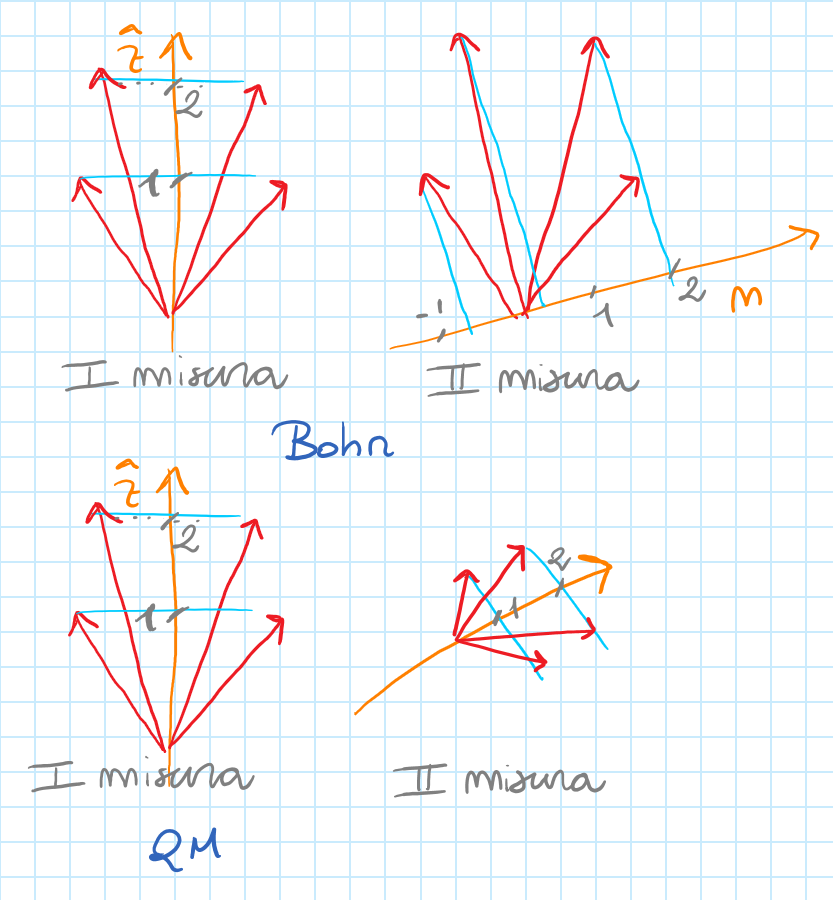
\includegraphics[scale=0.4]{Immagini/26_11/image001.png}

\tikzset{every picture/.style={line width=0.75pt}} %set default line width to 0.75pt        

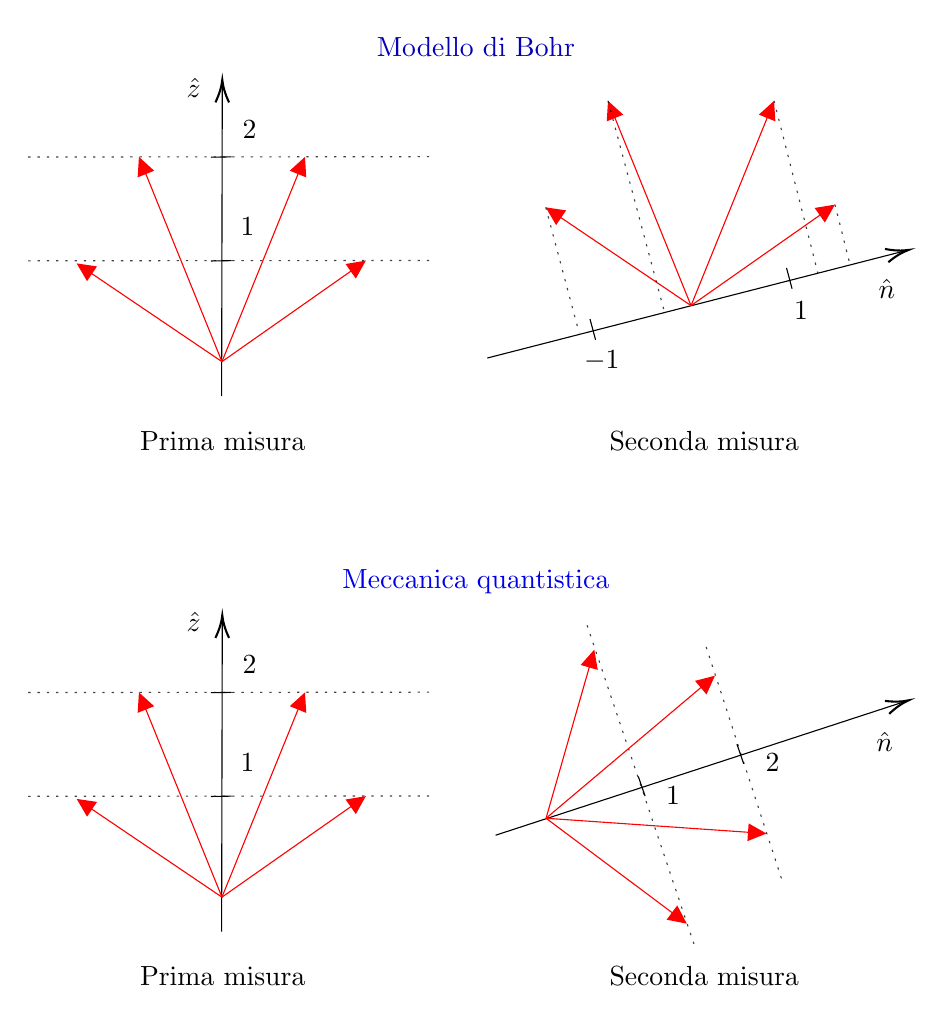
\begin{tikzpicture}[x=0.75pt,y=0.75pt,yscale=-1,xscale=1]
%uncomment if require: \path (0,512); %set diagram left start at 0, and has height of 512

%Straight Lines [id:da4395174486918325] 
\draw    (179.5,193.5) -- (179.83,43) ;
\draw [shift={(179.83,41)}, rotate = 450.13] [color={rgb, 255:red, 0; green, 0; blue, 0 }  ][line width=0.75]    (10.93,-3.29) .. controls (6.95,-1.4) and (3.31,-0.3) .. (0,0) .. controls (3.31,0.3) and (6.95,1.4) .. (10.93,3.29)   ;

%Straight Lines [id:da48343633533567787] 
\draw    (174.33,128.33) -- (184.33,128.17) ;


%Straight Lines [id:da7439374232299747] 
\draw    (174.33,78.33) -- (184.33,78.17) ;


%Straight Lines [id:da023005020016081623] 
\draw [color={rgb, 255:red, 0; green, 0; blue, 0 }  ,draw opacity=0.74 ] [dash pattern={on 0.84pt off 2.51pt}]  (86.33,78.25) -- (282.33,78.08) ;


%Straight Lines [id:da8196503395724821] 
\draw [color={rgb, 255:red, 0; green, 0; blue, 0 }  ,draw opacity=0.74 ] [dash pattern={on 0.84pt off 2.51pt}]  (86.33,128.25) -- (282.33,128.08) ;


%Straight Lines [id:da2056049527147128] 
\draw [color={rgb, 255:red, 255; green, 0; blue, 0 }  ,draw opacity=1 ]   (179.67,176.83) -- (247.36,129.32) ;
\draw [shift={(249,128.17)}, rotate = 504.93] [fill={rgb, 255:red, 255; green, 0; blue, 0 }  ,fill opacity=1 ][line width=0.75]  [draw opacity=0] (8.93,-4.29) -- (0,0) -- (8.93,4.29) -- cycle    ;

%Straight Lines [id:da23749320076574043] 
\draw [color={rgb, 255:red, 255; green, 0; blue, 0 }  ,draw opacity=1 ]   (179.67,176.83) -- (111.32,130.62) ;
\draw [shift={(109.67,129.5)}, rotate = 394.07] [fill={rgb, 255:red, 255; green, 0; blue, 0 }  ,fill opacity=1 ][line width=0.75]  [draw opacity=0] (8.93,-4.29) -- (0,0) -- (8.93,4.29) -- cycle    ;

%Straight Lines [id:da48502429041355355] 
\draw [color={rgb, 255:red, 255; green, 0; blue, 0 }  ,draw opacity=1 ]   (179.67,176.83) -- (140.42,80.02) ;
\draw [shift={(139.67,78.17)}, rotate = 427.93] [fill={rgb, 255:red, 255; green, 0; blue, 0 }  ,fill opacity=1 ][line width=0.75]  [draw opacity=0] (8.93,-4.29) -- (0,0) -- (8.93,4.29) -- cycle    ;

%Straight Lines [id:da3961417714512758] 
\draw [color={rgb, 255:red, 255; green, 0; blue, 0 }  ,draw opacity=1 ]   (179.67,176.83) -- (218.92,80.02) ;
\draw [shift={(219.67,78.17)}, rotate = 472.07] [fill={rgb, 255:red, 255; green, 0; blue, 0 }  ,fill opacity=1 ][line width=0.75]  [draw opacity=0] (8.93,-4.29) -- (0,0) -- (8.93,4.29) -- cycle    ;

%Straight Lines [id:da7687823680247343] 
\draw    (307.54,175.08) -- (508.56,123.5) ;
\draw [shift={(510.5,123)}, rotate = 525.61] [color={rgb, 255:red, 0; green, 0; blue, 0 }  ][line width=0.75]    (10.93,-3.29) .. controls (6.95,-1.4) and (3.31,-0.3) .. (0,0) .. controls (3.31,0.3) and (6.95,1.4) .. (10.93,3.29)   ;

%Straight Lines [id:da7153576437862126] 
\draw [color={rgb, 255:red, 0; green, 0; blue, 0 }  ,draw opacity=0.74 ] [dash pattern={on 0.84pt off 2.51pt}]  (445.67,51.17) -- (466.75,134) ;


%Straight Lines [id:da6014350597750142] 
\draw [color={rgb, 255:red, 0; green, 0; blue, 0 }  ,draw opacity=0.74 ] [dash pattern={on 0.84pt off 2.51pt}]  (475,101.17) -- (482.25,130) ;


%Straight Lines [id:da22855334364587865] 
\draw [color={rgb, 255:red, 255; green, 0; blue, 0 }  ,draw opacity=1 ]   (405.67,149.83) -- (473.36,102.32) ;
\draw [shift={(475,101.17)}, rotate = 504.93] [fill={rgb, 255:red, 255; green, 0; blue, 0 }  ,fill opacity=1 ][line width=0.75]  [draw opacity=0] (8.93,-4.29) -- (0,0) -- (8.93,4.29) -- cycle    ;

%Straight Lines [id:da6382566047761637] 
\draw [color={rgb, 255:red, 255; green, 0; blue, 0 }  ,draw opacity=1 ]   (405.67,149.83) -- (337.32,103.62) ;
\draw [shift={(335.67,102.5)}, rotate = 394.07] [fill={rgb, 255:red, 255; green, 0; blue, 0 }  ,fill opacity=1 ][line width=0.75]  [draw opacity=0] (8.93,-4.29) -- (0,0) -- (8.93,4.29) -- cycle    ;

%Straight Lines [id:da1767544477615266] 
\draw [color={rgb, 255:red, 255; green, 0; blue, 0 }  ,draw opacity=1 ]   (405.67,149.83) -- (366.42,53.02) ;
\draw [shift={(365.67,51.17)}, rotate = 427.93] [fill={rgb, 255:red, 255; green, 0; blue, 0 }  ,fill opacity=1 ][line width=0.75]  [draw opacity=0] (8.93,-4.29) -- (0,0) -- (8.93,4.29) -- cycle    ;

%Straight Lines [id:da0369041567294075] 
\draw [color={rgb, 255:red, 255; green, 0; blue, 0 }  ,draw opacity=1 ]   (405.67,149.83) -- (444.92,53.02) ;
\draw [shift={(445.67,51.17)}, rotate = 472.07] [fill={rgb, 255:red, 255; green, 0; blue, 0 }  ,fill opacity=1 ][line width=0.75]  [draw opacity=0] (8.93,-4.29) -- (0,0) -- (8.93,4.29) -- cycle    ;

%Straight Lines [id:da3701403896868616] 
\draw [color={rgb, 255:red, 0; green, 0; blue, 0 }  ,draw opacity=0.74 ] [dash pattern={on 0.84pt off 2.51pt}]  (365.67,51.17) -- (392.75,152.5) ;

%Straight Lines [id:da3562182437364947] 
\draw [color={rgb, 255:red, 0; green, 0; blue, 0 }  ,draw opacity=0.74 ] [dash pattern={on 0.84pt off 2.51pt}]  (335.67,102.5) -- (351.75,163) ;

%Straight Lines [id:da13653365906772086] 
\draw    (357,156.33) -- (359.67,166.33) ;

%Straight Lines [id:da8098653070285295] 
\draw    (451.67,131.67) -- (454.33,141.67) ;

%Straight Lines [id:da26221712769810845] 
\draw    (179.5,451.5) -- (179.83,301) ;
\draw [shift={(179.83,299)}, rotate = 450.13] [color={rgb, 255:red, 0; green, 0; blue, 0 }  ][line width=0.75]    (10.93,-3.29) .. controls (6.95,-1.4) and (3.31,-0.3) .. (0,0) .. controls (3.31,0.3) and (6.95,1.4) .. (10.93,3.29)   ;

%Straight Lines [id:da17449596529568234] 
\draw    (174.33,386.33) -- (184.33,386.17) ;

%Straight Lines [id:da6576782744524532] 
\draw    (174.33,336.33) -- (184.33,336.17) ;

%Straight Lines [id:da26817706480234316] 
\draw [color={rgb, 255:red, 0; green, 0; blue, 0 }  ,draw opacity=0.74 ] [dash pattern={on 0.84pt off 2.51pt}]  (86.33,336.25) -- (282.33,336.08) ;

%Straight Lines [id:da6900943454300643] 
\draw [color={rgb, 255:red, 0; green, 0; blue, 0 }  ,draw opacity=0.74 ] [dash pattern={on 0.84pt off 2.51pt}]  (86.33,386.25) -- (282.33,386.08) ;

%Straight Lines [id:da43880215320038074] 
\draw [color={rgb, 255:red, 255; green, 0; blue, 0 }  ,draw opacity=1 ]   (179.67,434.83) -- (247.36,387.32) ;
\draw [shift={(249,386.17)}, rotate = 504.93] [fill={rgb, 255:red, 255; green, 0; blue, 0 }  ,fill opacity=1 ][line width=0.75]  [draw opacity=0] (8.93,-4.29) -- (0,0) -- (8.93,4.29) -- cycle    ;

%Straight Lines [id:da18199577157737235] 
\draw [color={rgb, 255:red, 255; green, 0; blue, 0 }  ,draw opacity=1 ]   (179.67,434.83) -- (111.32,388.62) ;
\draw [shift={(109.67,387.5)}, rotate = 394.07] [fill={rgb, 255:red, 255; green, 0; blue, 0 }  ,fill opacity=1 ][line width=0.75]  [draw opacity=0] (8.93,-4.29) -- (0,0) -- (8.93,4.29) -- cycle    ;

%Straight Lines [id:da15939719614637227] 
\draw [color={rgb, 255:red, 255; green, 0; blue, 0 }  ,draw opacity=1 ]   (179.67,434.83) -- (140.42,338.02) ;
\draw [shift={(139.67,336.17)}, rotate = 427.93] [fill={rgb, 255:red, 255; green, 0; blue, 0 }  ,fill opacity=1 ][line width=0.75]  [draw opacity=0] (8.93,-4.29) -- (0,0) -- (8.93,4.29) -- cycle    ;

%Straight Lines [id:da9753617019587457] 
\draw [color={rgb, 255:red, 255; green, 0; blue, 0 }  ,draw opacity=1 ]   (179.67,434.83) -- (218.92,338.02) ;
\draw [shift={(219.67,336.17)}, rotate = 472.07] [fill={rgb, 255:red, 255; green, 0; blue, 0 }  ,fill opacity=1 ][line width=0.75]  [draw opacity=0] (8.93,-4.29) -- (0,0) -- (8.93,4.29) -- cycle    ;

%Straight Lines [id:da844222375866968] 
\draw    (311.5,405) -- (508.6,340.62) ;
\draw [shift={(510.5,340)}, rotate = 521.9100000000001] [color={rgb, 255:red, 0; green, 0; blue, 0 }  ][line width=0.75]    (10.93,-3.29) .. controls (6.95,-1.4) and (3.31,-0.3) .. (0,0) .. controls (3.31,0.3) and (6.95,1.4) .. (10.93,3.29)   ;

%Straight Lines [id:da3442233270834423] 
\draw    (380.26,376.69) -- (383.53,386.14) ;

%Straight Lines [id:da2882042278554833] 
\draw    (427.79,361.15) -- (431.05,370.61) ;

%Straight Lines [id:da592604983909238] 
\draw [color={rgb, 255:red, 0; green, 0; blue, 0 }  ,draw opacity=0.74 ] [dash pattern={on 0.84pt off 2.51pt}]  (412.98,314.29) -- (449.75,427.47) ;

%Straight Lines [id:da40350244649867273] 
\draw [color={rgb, 255:red, 0; green, 0; blue, 0 }  ,draw opacity=0.74 ] [dash pattern={on 0.84pt off 2.51pt}]  (355.6,303.84) -- (407.68,459.24) ;

%Straight Lines [id:da43189435972867307] 
\draw [color={rgb, 255:red, 255; green, 0; blue, 0 }  ,draw opacity=1 ]   (335.82,396.82) -- (402.02,446.41) ;
\draw [shift={(403.62,447.61)}, rotate = 216.82999999999998] [fill={rgb, 255:red, 255; green, 0; blue, 0 }  ,fill opacity=1 ][line width=0.75]  [draw opacity=0] (8.93,-4.29) -- (0,0) -- (8.93,4.29) -- cycle    ;

%Straight Lines [id:da10645710964392308] 
\draw [color={rgb, 255:red, 255; green, 0; blue, 0 }  ,draw opacity=1 ]   (335.82,396.82) -- (358.51,317.5) ;
\draw [shift={(359.06,315.58)}, rotate = 465.97] [fill={rgb, 255:red, 255; green, 0; blue, 0 }  ,fill opacity=1 ][line width=0.75]  [draw opacity=0] (8.93,-4.29) -- (0,0) -- (8.93,4.29) -- cycle    ;

%Straight Lines [id:da7643435946543784] 
\draw [color={rgb, 255:red, 255; green, 0; blue, 0 }  ,draw opacity=1 ]   (335.82,396.82) -- (415.65,329.44) ;
\draw [shift={(417.18,328.15)}, rotate = 499.83] [fill={rgb, 255:red, 255; green, 0; blue, 0 }  ,fill opacity=1 ][line width=0.75]  [draw opacity=0] (8.93,-4.29) -- (0,0) -- (8.93,4.29) -- cycle    ;

%Straight Lines [id:da4700730662028574] 
\draw [color={rgb, 255:red, 255; green, 0; blue, 0 }  ,draw opacity=1 ]   (335.82,396.82) -- (440.04,404.05) ;
\draw [shift={(442.03,404.19)}, rotate = 183.97] [fill={rgb, 255:red, 255; green, 0; blue, 0 }  ,fill opacity=1 ][line width=0.75]  [draw opacity=0] (8.93,-4.29) -- (0,0) -- (8.93,4.29) -- cycle    ;

% Text Node
\draw (166,45) node   {$\hat{z}$};
% Text Node
\draw (193,65) node   {$2$};
% Text Node
\draw (192,112) node   {$1$};
% Text Node
\draw (180,215) node  [align=left] {Prima misura};
% Text Node
\draw (412,215) node  [align=left] {Seconda misura};
% Text Node
\draw (302,25) node [color={rgb, 255:red, 0; green, 0; blue, 230 }  ,opacity=1 ] [align=left] {\textcolor[rgb]{0.02,0,0.71}{Modello di Bohr}};
% Text Node
\draw (500,142) node   {$\hat{n}$};
% Text Node
\draw (458.67,152.33) node   {$1$};
% Text Node
\draw (362.67,176.33) node   {$-1$};
% Text Node
\draw (166,302) node   {$\hat{z}$};
% Text Node
\draw (193,323) node   {$2$};
% Text Node
\draw (192,370) node   {$1$};
% Text Node
\draw (180,473) node  [align=left] {Prima misura};
% Text Node
\draw (412,473) node  [align=left] {Seconda misura};
% Text Node
\draw (302,283) node [color={rgb, 255:red, 0; green, 0; blue, 230 }  ,opacity=1 ] [align=left] {Meccanica quantistica};
% Text Node
\draw (397,386) node   {$1$};
% Text Node
\draw (445,370) node   {$2$};
% Text Node
\draw (499,360) node   {$\hat{n}$};
\end{tikzpicture}
\caption{Confronto tra modello semiclassico di Bohr e teoria quantistica. Nel primo caso si introduce \q{ad hoc} la quantizzazione del momento angolare, ma misure lungo assi diversi sono ancora considerate compatibili, e ciò crea problemi perché è impossibile che lo \textit{stesso vettore} abbia proiezioni \textit{quantizzate} lungo un qualsiasi asse (a meno che non sia il vettore nullo). La situazione è risolta in \MQ, dove misure di componenti diverse di $\vec{L}$ sono incompatibili, e fare una \textit{modifica} il risultato dell'altra.}
\end{figure}
Ipotizziamo infatti di misurare $\vec{L}\cdot \hat{z}$: otterremo allora un multiplo di $\hbar$, che per esempio sarà scelto tra $-2,-1,0,+1,+2$. Se ora misuriamo lungo $\hat{n}$ generico, se il momento ha la stessa direzione che abbiamo determinato prima, chiaramente possiamo scegliere $\hat{n}$ in modo che il risultato \textit{non possa essere un multiplo intero di $\hbar$}, ma ciò è in contrasto con gli esperimenti, dove comunque si osserva un valore multiplo intero di $\hbar$.\\
Classicamente non ha senso, e neanche nell'idea di Bohr, dove le \q{orbite} sono ancora \q{reali}, nel senso che \q{esistono} e non sono \textit{collassate}, ossia determinate, dall'atto di misura.\\
In \MQ, invece, fare la nuova misura lungo $\vec{n}$ è come se \q{ridefinisse} i vettori del momento in modo che le loro proiezioni lungo l'asse scelto siano multipli interi di $\hbar$. Ma questo si può fare perché \textit{non} si può mai misurare simultaneamente lungo due assi, dato che una misura irrimediabilmente modifica lo stato del sistema.
\end{itemize}

\subsection{Lo spin}%Inserire ref più specifica alla sezione [TO DO]
Nelle sezioni precedenti, abbiamo osservato che in \MQ $\vec{L}$ non è il più generale momento angolare, che invece è dato da $\vec{J}$, per cui valgono solo $[J_i, J_j]=i\hbar \epsilon_{ijk}J_k$, senza alcuna condizione sulle rotazioni di $2\pi$ che devono essere per forza equivalenti alla rotazione nulla.\\
Abbiamo\index{Spin!Origine} però determinato che gli autovettori comuni di $\vec{L}^{\,2}$ e $L_3$ dati da $\{\ket{l,m}, l\in \bb{N}, m \in \bb{Z}\cap [-l,l]\}$ costituiscono una \textbf{base} per la parte angolare di $L^2(\bb{R}^3, d^3x)$ su cui agiscono le rotazioni generate da $\vec{L}$.\\
Ma allora se $\vec{J}\neq \vec{L}$, si ha che $\vec{J}$ non può agire più solo\marginpar{$\vec{J}$ agisce su uno spazio di Hilbert \q{più grande}} sullo spazio di Hilbert $L^2(\bb{R}^3, d^3x)$, ma su uno spazio più grande, che sarà del tipo $L^2(\bb{R}^3, d^3x)\otimes \hs_s$.\\
Vediamo il perché. Supponiamo che $\vec{L}$ e $\vec{J}$ agiscano entrambi su $L^2(\bb{R}^3, d^3x)$. Le relazioni di commutazione per $\vec{L}$ sono date da:
\[
[L_i, X_l] = i\hbar \epsilon_{ilk} X_k; \qquad [L_i, P_l]=i\hbar \epsilon_{ilk} P_k
\]
E relazioni analoghe valgono anche per $\vec{J}$, dato che è anch'esso generatore delle rotazioni:
\begin{align*}
[J_i,X_l]=i\hbar \epsilon_{ilk} X_k; \qquad [J_i, P_l]=i\hbar \epsilon_{ilk} P_k
\end{align*}
Sottraendo i corrispettivi commutatori a membro giungiamo a:
\begin{align*}
[J_i-L_i, \vec{X}]=0 && [J_i-L_i, \vec{P}]=0
\end{align*}

In $L^2(\bb{R}^3)$ sappiamo però che $\{\vec{X},\vec{P}\}$ è un sistema \textit{irriducibile} di osservabili, e ogni osservabile che commuta con tutti gli elementi di tale sistema deve assumere autovalori che non dipendono in alcun modo dallo stato in cui è calcolata, e quindi è un multiplo dell'identità. Vale quindi:
\begin{align*}
J_i-L_i = c_i \bb{I} \Rightarrow J_i =L_i + c_i\bb{I}
\end{align*}

Ma allora otteniamo:
\[
[J_i, J_j]=[L_i + c_i \bb{I}, L_j + c_j \bb{I}]=i\hbar \epsilon_{ijk}L_k \neq i\hbar \epsilon_{ijk}J_k
\]
a meno che le $c_j = 0$, ma allora si avrebbe $\vec{J}=\vec{L}$, che è il contrario dell'ipotesi da cui siamo partiti.\\

 Deve esistere allora una nuova osservabile $\vec{S}$ che agisce su $\hs_s$ come momento angolare (ossia come \textit{generatore} delle rotazioni) in modo che:
\[
\vec{J}=\vec{L}\otimes \bb{I} + \bb{I}\otimes \vec{S} \rightsquigarrow \vec{J}=\vec{L}+\vec{S}
\]
Tale $\vec{S}$ è detto\textbf{ momento angolare di spin} o semplicemente spin, e valgono le analoghe proprietà del momento angolare: 
\begin{align*}
[S_i, S_j]&=i\hbar \epsilon_{ijk}S_k\\
\sigma(\vec{S}^{\,2}; S_3)&= \{\hbar^2 s(s+1), s\in \bb{N}/2; \hbar (s,s-1, \dots, -s)\}
\end{align*}

In particolare $s$ non è più vincolato a stare in $\bb{N}$, poiché non c'è più il vincolo fisico che una rotazione di $2\pi$ in $\hs_s$ che non è il \q{comune spazio classico} $L^2(\bb{R}^3)$ sia banale, ossia equivalente alla rotazione nulla.

\end{document}

